\documentclass[11pt,a4paper]{article}
\usepackage[margin=1in]{geometry}
\usepackage{booktabs}
\usepackage{xcolor}
\usepackage{tikz}
\usetikzlibrary{positioning}
\usepackage{enumitem}
\usepackage{fancyhdr}
\usepackage{titlesec}
\usepackage{colortbl}
\usepackage{array}

% Colors
\definecolor{primary}{RGB}{34, 87, 122}
\definecolor{secondary}{RGB}{87, 157, 28}
\definecolor{accent}{RGB}{242, 132, 65}
\definecolor{lightgray}{RGB}{245, 245, 245}

% Header styling
\pagestyle{fancy}
\fancyhf{}
\fancyhead[L]{\textcolor{primary}{\small Plant Health AI System}}
\fancyhead[R]{\textcolor{primary}{\small Technical Proposal}}
\fancyfoot[C]{\thepage}
\renewcommand{\headrulewidth}{0.5pt}
\setlength{\headheight}{14pt}

% Section styling
\titleformat{\section}{\Large\bfseries\color{primary}}{\thesection}{1em}{}
\titleformat{\subsection}{\large\bfseries\color{primary!80}}{\thesubsection}{1em}{}

\begin{document}

% Title Page
\begin{titlepage}
\centering
\vspace*{2cm}

{\Huge\bfseries\color{primary} Plant Health\\[0.3cm] Detection System\par}
\vspace{0.5cm}
{\Large\color{secondary} AI-Powered Analysis Platform\par}
\vspace{0.3cm}
{\large\color{accent} RGB Imaging Solution\par}

\vspace{2cm}

\begin{tikzpicture}
\draw[primary, line width=2pt] (0,0) -- (12,0);
\end{tikzpicture}

\vspace{1.5cm}

{\large\textbf{Technical Proposal}\par}
\vspace{0.5cm}
{\large Starting with Sugar Maple $\rightarrow$ Expanding to Multiple Species\par}

\vspace{3cm}

\begin{tabular}{rl}
\textbf{Author:} & Muhammad Danish Ashraf \\
\textbf{Date:} & February 2026 \\
\textbf{Sensor:} & RGB Camera \\
\end{tabular}

\vfill

\end{titlepage}

% Summary
\section{Overview}

This proposal outlines an AI-powered plant health detection system using RGB drone imagery. The system will be developed in phases, \textbf{starting with Sugar Maple as the base model}, then expanding to support multiple plant species.

\vspace{0.5cm}
\begin{center}
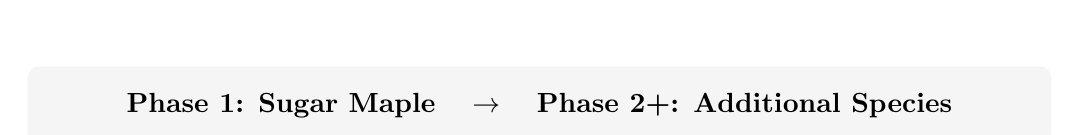
\begin{tikzpicture}
\node[fill=lightgray, rounded corners, minimum width=13cm, minimum height=1cm] {
\textbf{Phase 1: Sugar Maple} \quad $\rightarrow$ \quad \textbf{Phase 2+: Additional Species}
};
\end{tikzpicture}
\end{center}

\subsection{Problem Statement}

Traditional plant health assessment relies on manual inspection, which is:
\begin{itemize}[leftmargin=*]
\item \textbf{Time-intensive:} Ground-based surveys cover limited area per day
\item \textbf{Subjective:} Assessments vary between inspectors
\item \textbf{Reactive:} Problems often detected after significant damage occurs
\item \textbf{Costly:} Requires trained arborists for accurate diagnosis
\end{itemize}

\subsection{Proposed Solution}

An automated AI system that analyzes drone imagery to provide:
\begin{itemize}[leftmargin=*]
\item \textbf{Scalable coverage:} Analyze hundreds of trees per flight
\item \textbf{Consistent results:} Standardized detection criteria across all assessments
\item \textbf{Early detection:} Identify stress indicators before visible decline
\item \textbf{Actionable reports:} Prioritized recommendations for intervention
\end{itemize}

\section{Detection Modules}

The system comprises five detection modules that work together to provide comprehensive plant health assessment.

\subsection{Module 1: Species Detection}

Integration with 3rd party plant identification API to detect and confirm species before analysis.

\begin{center}
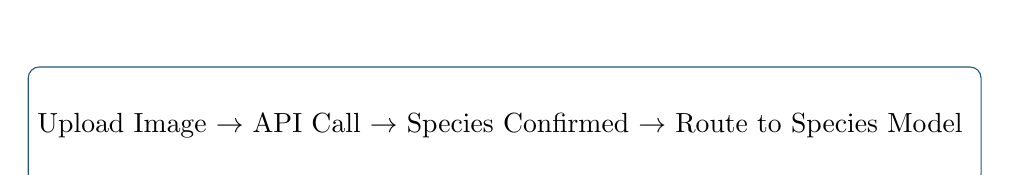
\begin{tikzpicture}
\node[draw=primary, rounded corners, minimum width=12cm, minimum height=1.5cm, align=center] {
Upload Image $\rightarrow$ API Call $\rightarrow$ Species Confirmed $\rightarrow$ Route to Species Model
};
\end{tikzpicture}
\end{center}

\textbf{Integration Details:}
\begin{itemize}[leftmargin=*]
\item API Provider: PlantNet or similar botanical identification service
\item Confidence threshold: $\geq$85\% required for automatic routing
\item Fallback handling: Manual review queue for low-confidence identifications
\item Caching: Species confirmed once per tree location to reduce API calls
\end{itemize}

\textbf{Supported Species (Phase 1):}
\begin{center}
\begin{tabular}{ll}
\toprule
\textbf{Common Name} & \textbf{Scientific Name} \\
\midrule
Sugar Maple & \textit{Acer saccharum} \\
\bottomrule
\end{tabular}
\end{center}

\subsection{Module 2: Maturity Classification}

Classify plants into growth stages based on crown/canopy characteristics.

\begin{center}
\begin{tabular}{ll}
\toprule
\textbf{Stage} & \textbf{Detection Method} \\
\midrule
Seedling & Small crown, simple structure \\
Sapling & Medium crown, developing canopy \\
Mature & Large crown, full canopy density \\
\bottomrule
\end{tabular}
\end{center}

\textbf{Technical Approach:}
\begin{itemize}[leftmargin=*]
\item Mask R-CNN for individual crown segmentation
\item Photogrammetric height estimation from drone imagery
\item Crown diameter and density analysis
\end{itemize}

\textbf{Classification Thresholds (Sugar Maple):}
\begin{center}
\begin{tabular}{lccc}
\toprule
\textbf{Stage} & \textbf{Height} & \textbf{Crown Diameter} & \textbf{DBH Est.} \\
\midrule
Seedling & $<$2m & $<$1.5m & $<$5cm \\
Sapling & 2--8m & 1.5--5m & 5--15cm \\
Mature & $>$8m & $>$5m & $>$15cm \\
\bottomrule
\end{tabular}
\end{center}

\textbf{Expected Accuracy:} 90\%+ classification accuracy based on crown characteristics visible in RGB imagery at 2--3cm GSD (Ground Sample Distance).

\subsection{Module 3: Leaf Disease Detection}

Detect and classify common foliar diseases using pattern recognition.

\textbf{For Sugar Maple (Phase 1):}
\begin{center}
\begin{tabular}{lll}
\toprule
\textbf{Disease} & \textbf{Visual Indicator} & \textbf{AI Method} \\
\midrule
Tar Spot & Black spots on leaves & Object detection (YOLO) \\
Anthracnose & Brown necrotic patches & Texture + color analysis \\
Leaf Spot & Circular brown lesions & Pattern matching \\
Powdery Mildew & White powdery coating & Albedo change detection \\
\bottomrule
\end{tabular}
\end{center}

\textbf{Expansion to Other Species:}
\begin{itemize}[leftmargin=*]
\item Train additional disease classes per species
\item Modular architecture allows adding new disease types
\item Transfer learning from base model speeds up training
\end{itemize}

\textbf{Severity Scoring:}
\begin{center}
\begin{tabular}{lcp{6cm}}
\toprule
\textbf{Level} & \textbf{Score} & \textbf{Criteria} \\
\midrule
None & 0 & No visible disease symptoms \\
Light & 1--2 & $<$10\% of visible foliage affected \\
Moderate & 3--4 & 10--30\% of visible foliage affected \\
Severe & 5 & $>$30\% of visible foliage affected \\
\bottomrule
\end{tabular}
\end{center}

\textbf{Output Format:}
\begin{itemize}[leftmargin=*]
\item Disease type with confidence score (0--100\%)
\item Affected area percentage estimate
\item Severity rating (0--5 scale)
\item Bounding boxes on detected lesions/symptoms
\end{itemize}

\subsection{Module 4: Vascular Disease Indicators}

Detect visual symptoms suggesting internal vascular problems.

\textbf{For Sugar Maple (Phase 1):}
\begin{center}
\begin{tabular}{ll}
\toprule
\textbf{Condition} & \textbf{Visible Symptoms Detected} \\
\midrule
Verticillium Wilt (Suspected) & Branch wilting, crown dieback, leaf browning \\
Eutypella Canker (Suspected) & Trunk deformation, bark anomalies \\
\bottomrule
\end{tabular}
\end{center}

\textbf{Detection Approach:}
\begin{itemize}[leftmargin=*]
\item Crown sector analysis for asymmetric dieback
\item Temporal comparison across survey dates
\item Oblique imagery for trunk-level symptoms
\end{itemize}

\textbf{Important Limitations:}
\begin{itemize}[leftmargin=*]
\item RGB imagery detects \textit{symptoms}, not pathogens directly
\item Results labeled as ``Suspected'' require ground verification
\item Internal vascular damage may not show external symptoms until advanced stages
\end{itemize}

\textbf{Recommendation Output:}
\begin{center}
\begin{tabular}{ll}
\toprule
\textbf{Confidence} & \textbf{Recommended Action} \\
\midrule
High ($>$80\%) & Priority ground inspection within 2 weeks \\
Medium (50--80\%) & Schedule ground inspection within 1 month \\
Low ($<$50\%) & Monitor in next survey cycle \\
\bottomrule
\end{tabular}
\end{center}

\subsection{Module 5: Damage Detection}

Identify structural damage visible in RGB imagery.

\begin{center}
\begin{tabular}{ll}
\toprule
\textbf{Damage Type} & \textbf{Detection Method} \\
\midrule
Dead Limb & Color difference (brown/gray vs green) \\
Broken Limb & Geometric anomaly in crown structure \\
Trunk Cavity & Visible external damage in oblique shots \\
Crown Asymmetry & Shape analysis indicating structural loss \\
Storm Damage & Multiple indicators combined detection \\
\bottomrule
\end{tabular}
\end{center}

\textbf{Risk Assessment Output:}
\begin{center}
\begin{tabular}{lp{8cm}}
\toprule
\textbf{Risk Level} & \textbf{Description} \\
\midrule
Low & Minor cosmetic damage, no structural concern \\
Medium & Moderate damage requiring monitoring \\
High & Significant structural damage, recommend arborist inspection \\
Critical & Imminent hazard, immediate attention required \\
\bottomrule
\end{tabular}
\end{center}

\subsection{Module 6: Size Estimation (Optional)}

Estimate physical dimensions using photogrammetry.

\begin{center}
\begin{tabular}{ll}
\toprule
\textbf{Metric} & \textbf{Method} \\
\midrule
Height & Digital Surface Model from drone imagery \\
Crown Width & Segmentation boundary measurement \\
Trunk Diameter & Allometric estimation from height + crown \\
Crown Volume & 3D reconstruction from overlapping imagery \\
\bottomrule
\end{tabular}
\end{center}

\textbf{Expected Accuracy:}
\begin{center}
\begin{tabular}{lcc}
\toprule
\textbf{Metric} & \textbf{Expected Accuracy} & \textbf{Requirements} \\
\midrule
Height & $\pm$0.5m & RTK-enabled drone, GCPs \\
Crown Width & $\pm$0.3m & 2cm GSD minimum \\
Trunk Diameter & $\pm$15\% & Allometric model calibration \\
\bottomrule
\end{tabular}
\end{center}

\textbf{Note:} Trunk diameter (DBH) estimation uses species-specific allometric equations. Accuracy improves with local calibration data.

\section{Data Requirements}

\subsection{Training Data}

For optimal model performance, the following data is required:

\begin{center}
\begin{tabular}{lcc}
\toprule
\textbf{Category} & \textbf{Minimum Images} & \textbf{Recommended} \\
\midrule
Healthy trees (various stages) & 200 & 500+ \\
Each disease type & 100 & 300+ \\
Damage examples & 50 & 150+ \\
Seasonal variation & 2 seasons & 4 seasons \\
\bottomrule
\end{tabular}
\end{center}

\subsection{Image Specifications}

\begin{center}
\begin{tabular}{ll}
\toprule
\textbf{Parameter} & \textbf{Requirement} \\
\midrule
Ground Sample Distance (GSD) & 1--3 cm/pixel recommended \\
Flight altitude & 30--60m AGL (species dependent) \\
Overlap & 75\% frontal, 65\% side minimum \\
Camera & RGB, minimum 20MP \\
Format & JPEG or TIFF, geotagged \\
Lighting & Overcast preferred, avoid harsh shadows \\
\bottomrule
\end{tabular}
\end{center}

\subsection{Annotation Requirements}

\begin{itemize}[leftmargin=*]
\item \textbf{Bounding boxes:} Individual tree crown delineation
\item \textbf{Polygons:} Disease lesion boundaries for training
\item \textbf{Labels:} Species, maturity stage, disease type, severity
\item \textbf{Metadata:} Date, location, ground truth verification where available
\end{itemize}

\textbf{Client Responsibility:} Provide raw drone imagery and any existing ground truth data. 

\section{Process Flow}

\subsection{Phase 1: Sugar Maple Base Model}

\begin{center}
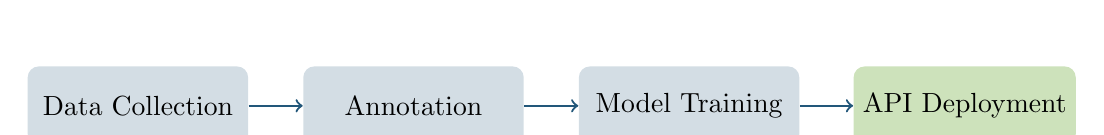
\begin{tikzpicture}[node distance=1cm, every node/.style={align=center}]
% Nodes
\node[fill=primary!20, rounded corners, minimum width=2.8cm, minimum height=1cm] (data) at (0,0) {Data Collection};
\node[fill=primary!20, rounded corners, minimum width=2.8cm, minimum height=1cm] (annotate) at (3.5,0) {Annotation};
\node[fill=primary!20, rounded corners, minimum width=2.8cm, minimum height=1cm] (train) at (7,0) {Model Training};
\node[fill=secondary!30, rounded corners, minimum width=2.8cm, minimum height=1cm] (deploy) at (10.5,0) {API Deployment};

% Arrows
\draw[->, thick, primary] (data) -- (annotate);
\draw[->, thick, primary] (annotate) -- (train);
\draw[->, thick, primary] (train) -- (deploy);
\end{tikzpicture}
\end{center}

\textbf{Phase 1 Milestones:}
\begin{center}
\begin{tabular}{lll}
\toprule
\textbf{Milestone} & \textbf{Week} & \textbf{Deliverable} \\
\midrule
M1: Data Ready & W3 & Annotated dataset complete \\
M2: Models Trained & W6 & All modules achieving target accuracy \\
M3: API Deployed & W8 & Functional API in staging environment \\
M4: Final Delivery & W10-12 & Production-ready system with documentation \\
\bottomrule
\end{tabular}
\end{center}

\subsection{Phase 2+: Multi-Species Expansion}

Once the Sugar Maple base model is complete, the system can expand to additional species.

\begin{center}
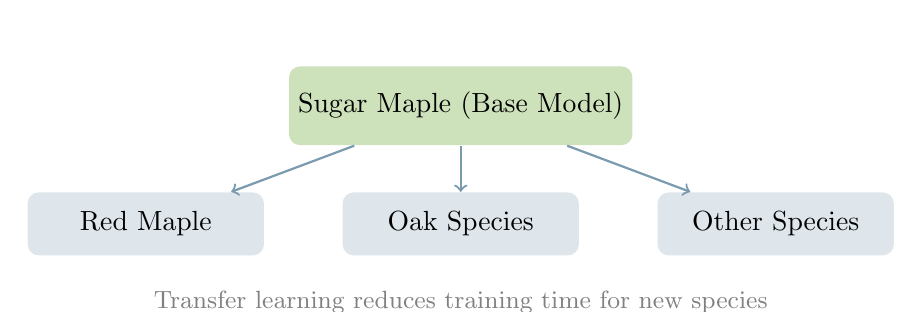
\begin{tikzpicture}
% Base
\node[fill=secondary!30, rounded corners, minimum width=4cm, minimum height=1cm, align=center] (base) at (0,0) {Sugar Maple (Base Model)};

% Expansions
\node[fill=primary!15, rounded corners, minimum width=3cm, minimum height=0.8cm] (sp1) at (-4,-1.5) {Red Maple};
\node[fill=primary!15, rounded corners, minimum width=3cm, minimum height=0.8cm] (sp2) at (0,-1.5) {Oak Species};
\node[fill=primary!15, rounded corners, minimum width=3cm, minimum height=0.8cm] (sp3) at (4,-1.5) {Other Species};

% Arrows
\draw[->, thick, primary!60] (base) -- (sp1);
\draw[->, thick, primary!60] (base) -- (sp2);
\draw[->, thick, primary!60] (base) -- (sp3);

% Label
\node[font=\small, color=gray] at (0,-2.5) {Transfer learning reduces training time for new species};
\end{tikzpicture}
\end{center}

\textbf{Expansion Process for Each New Species:}
\begin{enumerate}[leftmargin=*]
\item Collect species-specific training images
\item Annotate species-unique diseases and conditions
\item Fine-tune base model with new data
\item Validate and deploy updated API
\end{enumerate}

\section{Technical Architecture}

\subsection{System Components}

\begin{center}
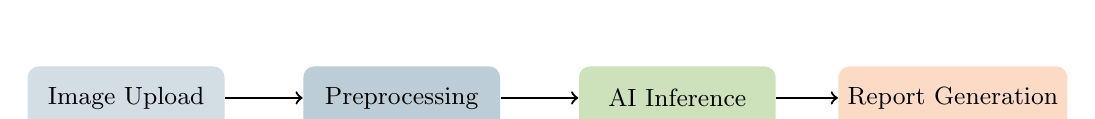
\begin{tikzpicture}[node distance=0.8cm, every node/.style={align=center, font=\small}]
% Input
\node[fill=primary!20, rounded corners, minimum width=2.5cm, minimum height=0.8cm] (input) at (0,0) {Image Upload};

% Processing
\node[fill=primary!30, rounded corners, minimum width=2.5cm, minimum height=0.8cm] (preprocess) at (3.5,0) {Preprocessing};
\node[fill=secondary!30, rounded corners, minimum width=2.5cm, minimum height=0.8cm] (inference) at (7,0) {AI Inference};
\node[fill=accent!30, rounded corners, minimum width=2.5cm, minimum height=0.8cm] (output) at (10.5,0) {Report Generation};

% Arrows
\draw[->, thick] (input) -- (preprocess);
\draw[->, thick] (preprocess) -- (inference);
\draw[->, thick] (inference) -- (output);
\end{tikzpicture}
\end{center}

\subsection{Technology Stack}

\begin{center}
\begin{tabular}{ll}
\toprule
\textbf{Component} & \textbf{Technology} \\
\midrule
Deep Learning Framework & PyTorch / TensorFlow \\
Object Detection & YOLO, Mask R-CNN \\
Image Processing & OpenCV, Pillow \\
API Framework & FastAPI (Python) \\
Database & PostgreSQL with PostGIS \\
Cloud Infrastructure & AWS / Azure / GCP (client choice) \\
Containerization & Docker \\
\bottomrule
\end{tabular}
\end{center}

\subsection{API Specification}

\textbf{Endpoints:}
\begin{itemize}[leftmargin=*]
\item \texttt{POST /analyze} -- Submit image for full analysis
\item \texttt{GET /results/\{id\}} -- Retrieve analysis results
\item \texttt{POST /batch} -- Submit multiple images for batch processing
\item \texttt{GET /health} -- Service health check
\end{itemize}

\textbf{Response Format:} JSON with structured results per module, including confidence scores, bounding boxes, and severity ratings.

\textbf{Authentication:} API key-based authentication with rate limiting.

\section{Team Structure}

\begin{center}
\begin{tabular}{lcp{6cm}}
\toprule
\textbf{Role} & \textbf{Count} & \textbf{Responsibilities} \\
\midrule
ML Engineer (Lead) & 1 & Architecture design, model optimization, API development \\
ML Engineer & 1 & Model training, evaluation, deployment support \\
Annotation Lead & 1 & Quality control, annotation guidelines, team coordination \\
Data Annotators & 2 & Image labeling, bounding box creation, data validation \\
\midrule
\textbf{Total} & \textbf{5} & \\
\bottomrule
\end{tabular}
\end{center}

\section{Quality Assurance}


\subsection{Testing Protocol}

\begin{enumerate}[leftmargin=*]
\item \textbf{Unit Testing:} Individual model component validation
\item \textbf{Integration Testing:} End-to-end pipeline verification
\item \textbf{Field Validation:} Testing on new imagery not used in training
\item \textbf{Expert Review:} Arborist validation of sample outputs
\end{enumerate}

\subsection{Continuous Improvement}

\begin{itemize}[leftmargin=*]
\item Feedback loop for misclassifications to improve model
\item Quarterly model retraining with accumulated data
\item Version control for all model iterations
\end{itemize}

\section{Timeline}

\begin{center}
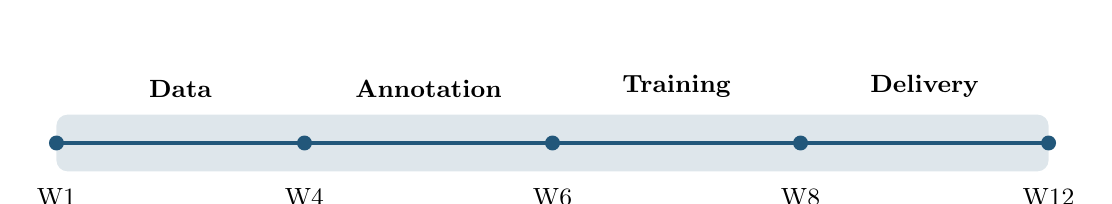
\begin{tikzpicture}[scale=0.9]
% Timeline bar
\fill[primary!15, rounded corners] (0,-0.4) rectangle (14,0.4);
\draw[primary, line width=1.5pt] (0,0) -- (14,0);

% Week markers
\foreach \x/\w in {0/W1, 3.5/W4, 7/W6, 10.5/W8, 14/W12} {
  \fill[primary] (\x,0) circle (3pt);
  \node[below, font=\small] at (\x,-0.5) {\w};
}

% Phases
\node[above, font=\small\bfseries] at (1.75,0.5) {Data};
\node[above, font=\small\bfseries] at (5.25,0.5) {Annotation};
\node[above, font=\small\bfseries] at (8.75,0.5) {Training};
\node[above, font=\small\bfseries] at (12.25,0.5) {Delivery};
\end{tikzpicture}
\end{center}

\section{Investment}

\begin{center}
\renewcommand{\arraystretch}{1.4}
\begin{tabular}{|l|r|}
\hline
\rowcolor{primary!20}
\textbf{Module} & \textbf{Cost (USD)} \\
\hline
Species Detection (3rd Party API) & Included \\
\hline
Maturity Classification & \$1,633 \\
\hline
Leaf Disease Detection (4 types) & \$2,100 \\
\hline
Vascular Disease Indicators & \$1,633 \\
\hline
Damage Detection & \$1,167 \\
\hline
Size Estimation & \$467 \\
\hline
\rowcolor{accent!20}
\textbf{Total (Phase 1 - Sugar Maple)} & \textbf{\$7,000} \\
\hline
\end{tabular}
\end{center}

\vspace{0.3cm}
\begin{center}
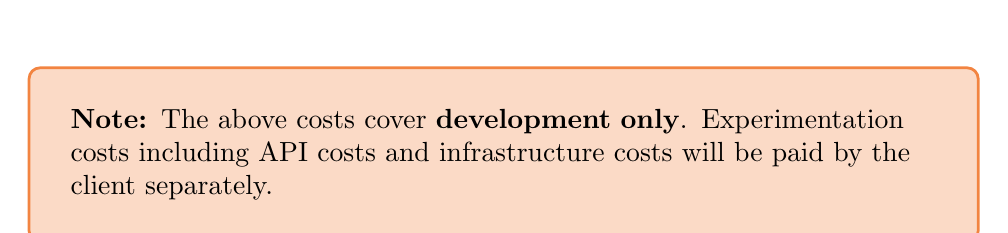
\begin{tikzpicture}
\node[fill=accent!30, rounded corners, minimum width=12cm, text width=11cm, align=left, inner sep=15pt, draw=accent, line width=1pt] {
\textbf{Note:} The above costs cover \textbf{development only}. Experimentation costs including API costs and infrastructure costs will be paid by the client separately.
};
\end{tikzpicture}
\end{center}
\vspace{0.3cm}

\begin{center}
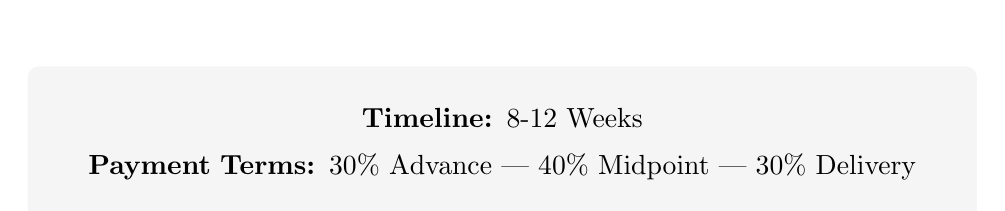
\begin{tikzpicture}
\node[fill=lightgray, rounded corners, minimum width=12cm, text width=11cm, align=center, inner sep=15pt] {
\textbf{Timeline:} 8-12 Weeks\\[5pt]
\textbf{Payment Terms:} 30\% Advance | 40\% Midpoint | 30\% Delivery
};
\end{tikzpicture}
\end{center}

\vspace{0.5cm}

\textbf{Future Species Expansion:} Pricing for additional species will be quoted separately based on disease complexity and annotation requirements. Transfer learning from the base model significantly reduces cost for subsequent species.

\section{Deliverables}

Upon project completion, the following will be delivered:

\begin{enumerate}[leftmargin=*]
\item \textbf{Trained AI Models}
\begin{itemize}
\item Maturity classification model (Sugar Maple)
\item Leaf disease detection model (4 disease types)
\item Vascular disease indicator model
\item Damage detection model
\item Size estimation model
\end{itemize}

\item \textbf{REST API Service}
\begin{itemize}
\item Dockerized deployment package
\item API documentation (OpenAPI/Swagger)
\item Sample client code (Python, JavaScript)
\end{itemize}

\item \textbf{Documentation}
\begin{itemize}
\item System architecture documentation
\item Model training methodology
\item Integration guide
\item User manual
\end{itemize}

\item \textbf{Support}
\begin{itemize}
\item 30-day post-deployment support
\item Bug fixes during support period
\item Knowledge transfer session (2 hours)
\end{itemize}
\end{enumerate}

\section{Assumptions \& Dependencies}

\subsection{Assumptions}

\begin{itemize}[leftmargin=*]
\item Client will provide sufficient training imagery meeting specified requirements
\item Drone imagery will be captured following recommended flight parameters
\item Access to subject matter expert (arborist) for validation queries
\item Stable internet connection for API deployment and testing
\end{itemize}

\subsection{Dependencies}

\begin{itemize}[leftmargin=*]
\item Third-party species identification API availability and pricing
\item Cloud infrastructure provisioning (client or provided)
\item Timely feedback on validation results during development
\end{itemize}

\subsection{Out of Scope}

\begin{itemize}[leftmargin=*]
\item Drone hardware or flight operations
\item Multispectral or hyperspectral imagery analysis
\item Real-time streaming video analysis
\item Mobile application development
\item Root disease detection (not visible in aerial imagery)
\end{itemize}

\section{Next Steps}

\begin{enumerate}[leftmargin=*]
\item \textbf{Proposal Acceptance:} Review and sign-off on scope and pricing
\item \textbf{Data Assessment:} Evaluate existing imagery and identify gaps
\item \textbf{Kickoff Meeting:} Align on timeline, communication, and milestones

\end{enumerate}

\vfill

\begin{center}
\textcolor{primary}{\rule{8cm}{0.5pt}}\\[0.3cm]
\textit{For questions or clarifications, please contact us.}
\end{center}

\end{document}
